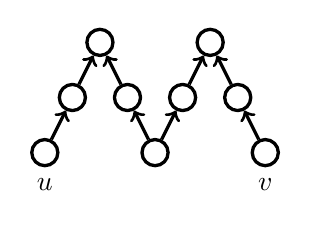
\begin{tikzpicture}[
    scale=0.35,
    line width=1.2pt
]
   % \node at (-4,-2) {\(F_2\)};
            
    \node[circle, draw=black, fill=white, label=below:{\(u\)}]
            (q0) at (4,-4) {};
    \node[circle, draw=black, fill=white, label=below:{}]
            (q1) at (8,-4) {};
    \node[circle, draw=black, fill=white, label=below:{\(v\)}]
            (q2) at (12,-4) {};
    \node[circle, draw=black, fill=white, label=below:{}]
            (q3) at (5,-2) {};
    \node[circle, draw=black, fill=white, label=below:{}]
            (q4) at (7,-2) {};
    \node[circle, draw=black, fill=white, label=below:{}]
            (q5) at (9,-2) {};
    \node[circle, draw=black, fill=white, label=below:{}]
            (q6) at (11,-2) {};
    \node[circle, draw=black, fill=white, label=below:{}]
        (q7) at (6,0) {};
    \node[circle, draw=black, fill=white, label=below:{}]
        (q8) at (10,0) {};   
        
    \draw[->] (q0) -- (q3);
    \draw[->] (q3) -- (q7);
    \draw[->] (q4) -- (q7);
    \draw[->] (q1) -- (q4);
    \draw[->] (q1) -- (q5);
    \draw[->] (q2) -- (q6);
    \draw[->] (q5) -- (q8);
    \draw[->] (q6) -- (q8);
\end{tikzpicture}